\chapter{Présentation du cadre du projet}
\section*{Introduction}
Ce chapitre a pour objectif de situer notre travail par rapport à son cadre général.
Nous commençons, tout d’abord, par la présentation de l'organisme d'accueil,
puis nous passons à des notions fondamentales relatives aux API .
Ensuite, nous abordons l'étude de marché et concluons par l'analyse de l'existant ainsi que la méthodologie et le langage de modélisation adoptés.


\section{Présentation de la société}
\subsection{Présentation générale }
Fondée en 2002, Vermeg est une entreprise off-shore comptant plus de 1600 collaborateurs, elle
est indépendante de la société mère BFI établie en 1994.
Vermeg dispose d'une expertise en monétique et en édition de logiciels bancaires et financiers, et offre une large gamme de logiciels pour les différents tiers des institutions financières concernés par le traitement des titres. \\
Les produits que Vermeg offre, sont utilisés dans dix-huit différents pays à travers trois continents. \\
la figure 1.1 représente la dispersion géographique de ses différents clients. \cite[]{vermeg}
\begin{figure}[H]    
    \centering
        \frame{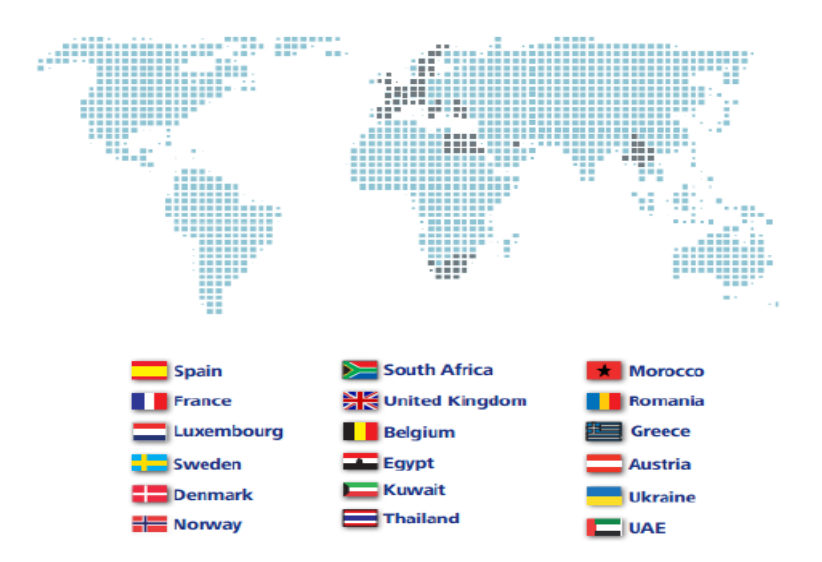
\includegraphics[width=0.9\columnwidth]{LesclientsdeVermegdanslemonde.png}}
        \caption{Les clients de Vermeg dans le monde }
        \label{fig:logo_tt}
    \end{figure}
\pagebreak
\subsection{Départements de Vermeg }
Les principaux départements  de Vermeg sont: \cite[]{vermeg}
\begin{itemize}
    \item \textbf{Recherche et Développement:} Se concentre sur l'innovation et le développement de nouvelles technologies et solutions.
    \item \textbf{Technologie et Développement de Produits :} Responsable de la conception, du  développement et de la maintenance des produits logiciels.
    \item \textbf{Ventes et Marketing :} Chargé de la promotion des produits et des services, de la gestion des relations clients et de l'acquisition de nouveaux clients.
    \item \textbf{Support Client et Services Professionnels :} Offre une assistance technique et des services de consultation aux clients.
    \item \textbf{Ressources Humaines :} Gère le recrutement, la formation, et le développement des employés ainsi que les relations de travail.
    \item \textbf{Finance et Comptabilité :} Gère les finances de l'entreprise, y compris la comptabilité, la gestion des budgets et les rapports financiers.
    \item \textbf{Gestion de Projet :} Assure la planification, l'exécution et la clôture des projets en respectant les délais et les budgets.
    \item \textbf{Qualité et Conformité :} Veille à ce que les produits et services répondent aux normes de qualité et aux réglementations en vigueur.
\end{itemize} 
Ces départements collaborent pour fournir des solutions technologiques complètes et innovantes aux clients de Vermeg dans les secteurs financiers et d'assurance. \\ 
Notre stage s'est effectué au sein du département Recherche et Développement.
\subsection{Services }
     L'activité de Vermeg s'articule principalement autour de quatre axes : \cite[]{vermeg}
    \begin{itemize}
        \item Assurance : couverture d’assurance individuelle ou de groupe pour l’épargne et la santé.
        \item Gestion de richesses et d’actifs : gestion des décisions financières dédiée aux besoins spécifiques de gestion du patrimoine.
        \item Marché financier et services de sécurité.
        \item Services financiers digitaux : numérisation des processus financiers et analyse des données sensibles.
    \end{itemize} 
    \pagebreak

    Vermeg fournit à ses clients un ensemble de logiciels spécialisés dans le domaine financier tels que :
    \begin{itemize}
        \item MEGARA (Securities processing) : La suite MEGARA est une plateforme modulaire pour le traitement des titres destinée essentiellement aux institutions financières qui propose un nombre de modules pouvant être implémentés séparément.
        \item PALMYRA : est un framework JEE compatible SOA (architecture orientée service) qui incorpore des composants ainsi que des services web réutilisables. L’implémentation de services web réutilisables permettant de développer des logiciels de meilleure qualité en temps réduit dont l’architecture est basée sur un client léger.
        \item SOLIFE : Une solution d’administration de polices d’assurance vie et un portail web à destination des clients finaux/brokers.
        \item SOLIAM : est une solution de gestion de portefeuilles pour les gestionnaires d’actifs institutionnels de fortune. Ayant une présence internationale en Belgique, France, Irlande, Luxembourg, Pays-Bas, Suisse, Royaume-Uni, Tunisie et des clients dans plus de 23 pays, VermegLife et Soliam sont considérés comme les deux produits phares de Vermeg BSB.
    \end{itemize} 
    
Maintenant que nous avons exploré la structure, les départements et les services de l'entreprise d'acceuil, et étant donné que Vermeg développe de nombreuses API et que notre projet s'inscrit dans ce contexte, nous allons aborder les concepts clés liés aux API.   

\section{Concepts clés autour des API}
Les API sont devenues des éléments essentiels du développement web moderne, permettant aux applications de communiquer et de partager des données. C’est pourquoi cette partie s'attache à présenter les fondements des API, leur documentation ainsi que le concept d'une marketplace d'API.
\subsection{Les Fondements des API }

    \subsubsection{Définition d'une API }
    Une API (Application Programming Interface) permet de rendre disponibles les données ou les fonctionnalités d’une application existante afin que d’autres applications les utilisent. Elle facilite le partage et l’intégration de fonctionnalités dans des architectures existantes. En pratique, une API agit comme un pont d'accès vers une fonction spécifique gérée par une entité distincte. \cite[]{DefAPI}
\pagebreak  
    \subsubsection{Fonctionnement d'une API }
    Une API fonctionne généralement selon le principe requête-réponse : 
    \begin{itemize}
        \item Requête: Le client envoie une requête à l'API, en précisant l'action souhaitée et les données nécessaires. 
        \item Réponse: L'API traite la requête et envoie une réponse au client, contenant les données ou les résultats de l'action demandée.
    \end{itemize} 

    \subsubsection{Types d'API}
    Les interfaces de programmation d’applications ne sont pas toutes créées de la même manière. Chaque type d’API a une utilité spécifique et s’intègre de manière différente dans l’écosystème des applications et des services. Voici les principaux types d'API selon les styles d’architecture : \\
    \textbf{a. API REST (Representational State Transfer) } \\
    Une API Rest est caractérisée par \cite[]{APIRest}:
    \begin{itemize}
        \item Architecture client-serveur sans état
        \item Accès aux ressources via des URL et des méthodes HTTP (GET, POST, PUT, DELETE)
        \item Formats de données courants : JSON, XML
        \item Facile à utiliser et à comprendre
        \item Flexible et évolutive  
    \end{itemize} 
    
    \textbf{b. API SOAP (Simple Object Access Protocol)  } \\
    Une API SOAP est caractérisée par \cite[]{APISOAP}:
    \begin{itemize}
        \item 	Architecture orientée service basée sur XML
        \item Utilisation de messages structurés et de protocoles web
        \item Norme plus complexe et plus lourde que REST
        \item Adaptée aux applications d'entreprise nécessitant une sécurité et une fiabilité élevées   
    \end{itemize} 

    \textbf{c. API RPC (Remote Procedure Call):} \\
    Une API RPC est caractérisée par  \cite[]{APIRPCGraphql}:
    \begin{itemize}
        \item Exécution des fonctions à distance sur un autre serveur
        \item Utilisation des protocoles spécifiques comme XML-RPC ou JSON-RPC
        \item Moins répandue que REST et SOAP, mais utile pour certaines applications telles que les systèmes distribués, les microservices, et les environnements nécessitant des appels de procédure rapides et directs  
    \end{itemize} 

    \textbf{d. API GraphQL } \\
    Une API graphQL est caractérisée par \cite[]{APIRPCGraphql}:
    \begin{itemize}
        \item Requêtes basées sur un schéma flexible
        \item Permet de récupérer des données précises et structurées
        \item Plus récent et plus moderne que REST et SOAP
        \item 	A Gagné en popularité pour son efficacité et sa flexibilité  
    \end{itemize} 

    \subsubsection{Structure d'une API}
    La structure d'une API comprend plusieurs éléments essentiels qui facilitent la communication entre le client et le serveur. Voici les composants :

    \begin{itemize}
        \item  \textbf{Endpoint : } C'est l'URL à laquelle l'API peut être accédée. Chaque endpoint correspond à une fonction spécifique de l'API. Par exemple, https://api.example.com/users peut être un endpoint pour accéder aux utilisateurs.
        \item \textbf{Méthodes HTTP : } Les actions possibles sur les ressources sont définies par les méthodes HTTP. Les plus courantes sont : GET, POST, PUT, DELETE
        \item  \textbf{En-têtes (Headers) : }  Informations supplémentaires envoyées avec les requêtes et les réponses HTTP, souvent utilisées pour l'authentification, la gestion du cache, le contrôle des formats de données, etc.
        \item \textbf{ Paramètres :}
        \begin{itemize}
            \item    \textbf{Path Parameters} Inclus dans l'URL pour spécifier une ressource particulière, par exemple, /users/{id}.
            \item \textbf{Query Parameters :} Inclus dans l'URL après le symbole \texttt{?} pour filtrer ou modifier la requête, par exemple, \texttt{?sort=asc\&limit=10}.
            \item  \textbf{Body Parameters}  Paramètres de corps (Body Parameters) : Utilisés principalement avec POST et PUT pour envoyer des données au serveur dans le corps de la requête.
        \end{itemize}
        \item  \textbf{Réponses:} Responses: Les réponses d'une API incluent le code de statut HTTP (par exemple, 200 pour le succès, 404 pour non trouvé, 500 pour une erreur serveur) et le corps de la réponse contenant les données ou les messages d'erreur
    \end{itemize} 
    
    
    Maintenant que nous avons examiné les fondements et les types d'API, il est essentiel de comprendre l'importance de la documentation qui est un élément crucial pour garantir la bonne utilisation et intégration d'une API.

    \subsection{Documentation d'une API }
    La documentation d'une API fournit aux développeurs et aux utilisateurs les clés pour exploiter pleinement le potentiel d'une API. En détaillant les endpoints, les méthodes, les paramètres, les réponses, les processus d'authentification, les exemples d'utilisation et la gestion des erreurs, elle éclaire les fonctionnalités de l'API et facilite son adoption.
    \subsubsection{Choix de la documentation  }
    Dans le domaine de la documentation des API, plusieurs formats sont utilisés, tels que Swagger/ OpenAPI, RAML, API Blueprint . Cependant, Swagger/OpenAPI est, en effet, l'un des formats les plus courants et les plus populaires.
    \subsubsection{Swagger/OpenAPI }

    Swagger a débuté comme un ensemble d'outils open-source développés par SmartBear Software pour simplifier la conception et la documentation des API RESTful. Avec le temps, il s'est transformé en un ensemble de spécifications et de formats permettant de décrire les API de manière claire et cohérente. En 2015, SmartBear Software a cédé la spécification Swagger à la fondation OpenAPI Initiative, qui l'a renommée OpenAPI Specification (OAS).
    Cette transition a élevé OpenAPI au rang de norme de l'industrie pour la documentation des API, offrant un standard largement adopté pour décrire les API de manière précise et uniforme. \cite[]{Swagger}

    \subsubsection{Caractéristiques d'un fichier Swagger/OpenAPI  }
    OpenAPI est une spécification de description d'API ouverte et standardisée. Elle permet de décrire les fonctionnalités d'une API de manière détaillée, notamment les endpoints, les paramètres, les réponses, etc… \\
    OpenAPI fournit un format standardisé pour la documentation des API. Les développeurs utilisent des fichiers au format JSON ou YAML pour décrire les API de manière claire et compréhensible.\cite[]{Swagger} \\
   La figure suivante présente un extrait d'un fichier swagger.
    \begin{figure}[H]    
    \centering
        \frame{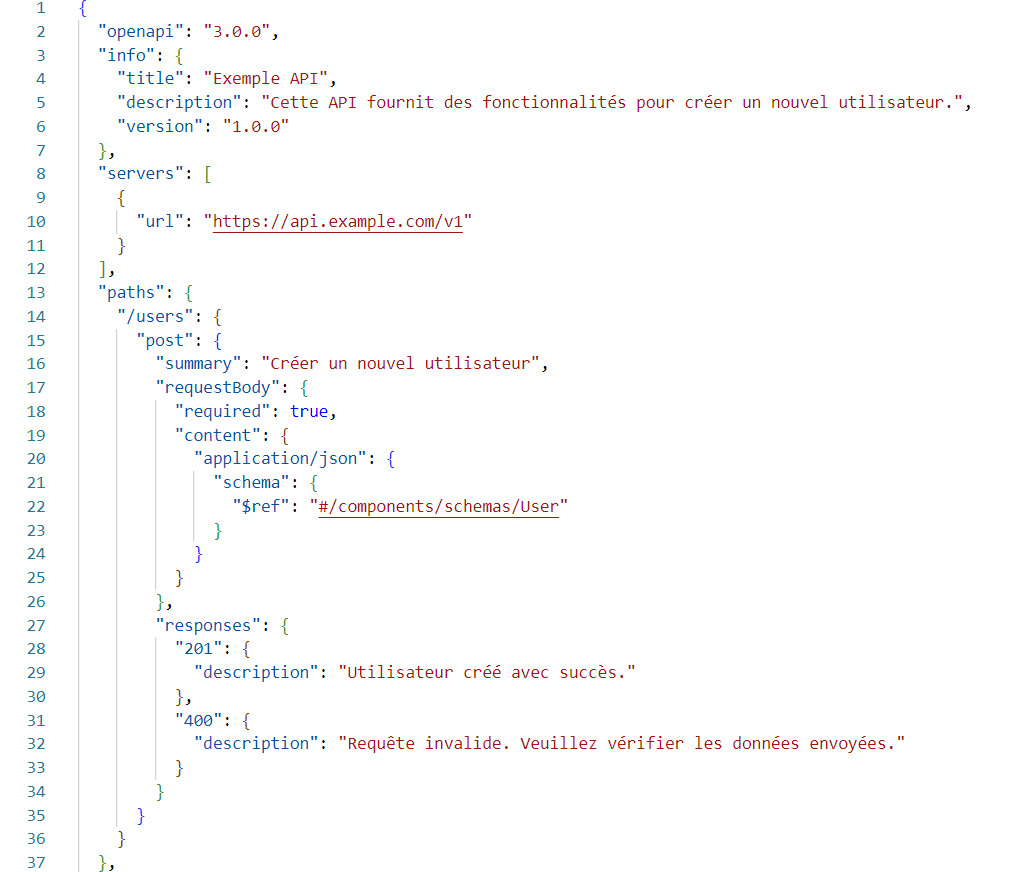
\includegraphics[width=1\columnwidth]{exemplefichierswagger.png}}
        \caption{Exemple de fichier swagger }
        \label{fig:logo_tt}
    \end{figure}
    Ce fichier Swagger décrit une API qui permet de créer un nouvel utilisateur via la méthode POST. 
    Lorsqu'un utilisateur est créé avec succès, la réponse sera un code 201 avec un message indiquant le succès de l'opération. 
    En cas de requête invalide, la réponse sera un code 400 avec un message informant l'utilisateur de vérifier les données envoyées. 
    \subsubsection{Avantages de Swagger/OpenAPI} 
        OpenAPI offre une documentation claire et cohérente pour les API, favorisant ainsi l'assimilation et l'adoption grâce à une documentation bien structurée. De plus, en adoptant OpenAPI, les organisations contribuent à la standardisation et à l'interopérabilité des API, simplifiant ainsi leur intégration avec différentes applications et systèmes. \\
        Bien que d'autres standards de documentation d'API, tels que RAML et API Blueprint, existent, Swagger et OpenAPI sont généralement préférés dans l'industrie en raison de leur large adoption, de leur écosystème d'outils et d'intégrations riches, ainsi que de leur soutien actif de la communauté.\cite[]{AvantageSwagger} 

    \subsubsection{Les outils de Swagger/OpenAPI }
    Plusieurs outils sont utilisés dans l'écosystème Swagger, tels que Swagger UI, Swagger Codegen et Swagger Editor. Swagger UI est utilisé pour afficher une interface interactive permettant aux développeurs et aux utilisateurs d'explorer facilement les endpoints, les paramètres et les réponses de l'API, améliorant ainsi la compréhension de son fonctionnement et favorisant son adoption.\cite[]{Swagger}
   
    \begin{figure}[H]    
        \centering
            \frame{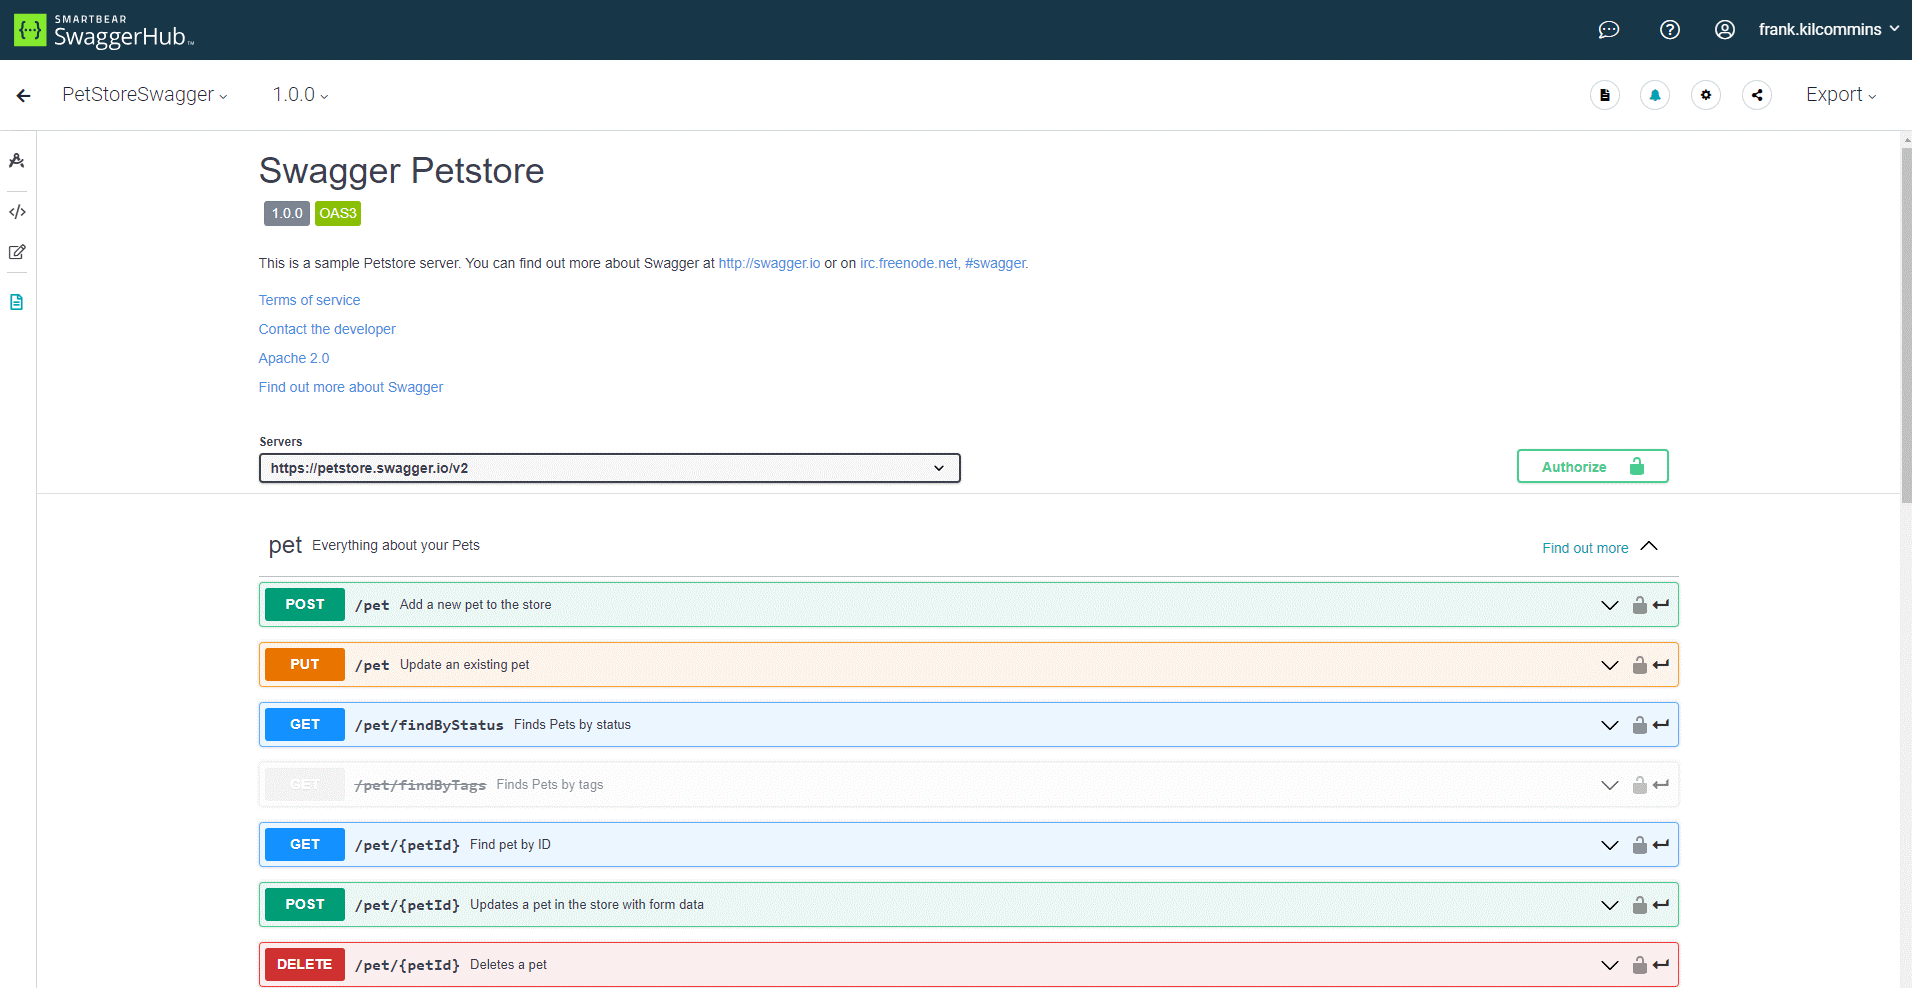
\includegraphics[width=1\columnwidth]{InterfacedeSwaggerUI.png}}
            \caption{Interface de Swagger UI }
            \label{fig:logo_tt}
        \end{figure}

       % Après avoir exploré la documentation détaillée des API, il est important de mentionner que Vermeg dispose de nombreuses API qui ne sont pas encore partagées ou pleinement utilisées. C'est pourquoi nous avons eu l'idée de créer un marketplace d'API où ces API peuvent être commercialisées et utilisées. Passons maintenant à l'exploration du concept de marketplace d'API, un espace dédié à la découverte, à l'échange et à la monétisation de ces API essentielles pour répondre aux besoins variés des développeurs et des entreprises.

       La documentation détaillée des API est cruciale pour leur adoption et leur utilisation efficace. Elle fournit une compréhension claire des fonctionnalités et des usages des API, facilitant leur intégration dans divers projets de développement. Cependant, la documentation seule ne suffit pas toujours à rendre les API largement accessibles. C'est ici qu'intervient le concept de marketplace d'API, qui offre un espace centralisé où les développeurs peuvent non seulement trouver et utiliser des API, mais aussi les commercialiser et les monétiser publiquement, rendant ainsi les API plus accessibles et favorisant une adoption plus large.

\pagebreak

\subsection{ MarketPlace d'API }

    \subsubsection{ Définition d'une marketPlace d’API} 


    Une marketplace d'API est une plateforme en ligne dédiée aux développeurs et aux entreprises pour découvrir, acheter, vendre et intégrer des API. \\
        Elle facilite l'échange de services et de données entre différents systèmes en offrant une plateforme centralisée pour les API, permettant ainsi aux fournisseurs de monétiser leurs API et aux consommateurs de trouver facilement les solutions dont ils ont besoin comme l’illustre la figure suivante:
        \begin{figure}[H]    
            \centering
                \frame{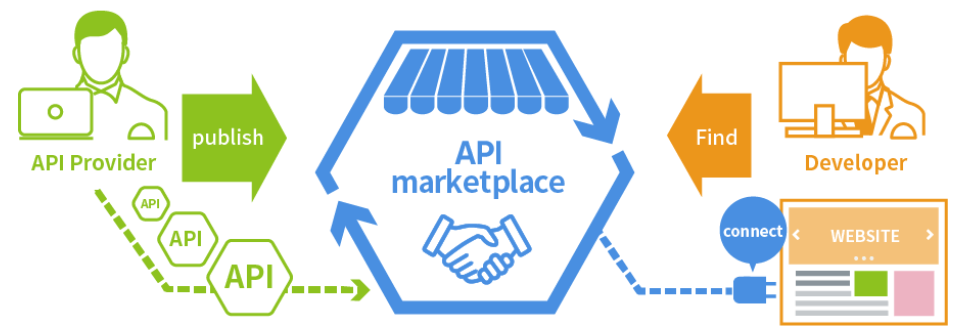
\includegraphics[width=0.8\columnwidth]{ProcessusdemarketplacedAPI.png}}
                \caption{ Fonctionnement d’une marketplace d’API \cite[]{marketplaceAPI} }
                \label{fig:logo_tt}
        \end{figure}
    \subsubsection{ Fonctionnalités d'une marketPlace d’API}

    Les fonctionnalités d'une API Marketplace varient d'une plateforme à l'autre, mais les plus courantes incluent :	
    \begin{itemize}
        \item    \textbf{Recherche d'APIs :}  Les développeurs d'applications peuvent rechercher des APIs par nom, par catégorie, par fonctionnalité, etc.
        \item  \textbf{Consultation des détails des APIs : }Les développeurs d'applications peuvent consulter les détails d'une API, tels que sa documentation, ses exemples de code, ses tarifs, etc.
        \item \textbf{Abonnement aux APIs : }Les développeurs d'applications peuvent s'abonner aux APIs qu'ils souhaitent utiliser.
        \item \textbf{Consommation des APIs :} Les développeurs d'applications peuvent utiliser les APIs auxquelles ils sont abonnés pour ajouter des fonctionnalités à leurs applications.
        \item  \textbf{Gestion des APIs :} Les fournisseurs d'API peuvent gérer leurs APIs sur la plateforme, en modifiant leurs informations, en ajoutant de nouvelles fonctionnalités et endpoints, etc.
    \end{itemize}
\pagebreak

    \subsubsection{ Avantages d'une marketPlace d’API}
Les API Marketplaces offrent plusieurs avantages tant pour les fournisseurs d'API que pour les développeurs d'applications : \\
\textbf{Pour les Fournisseurs d'API :} 
\begin{itemize}
    \item Augmentation de la visibilité de leurs APIs, ce qui peut conduire à une plus grande adoption et utilisation.
    \item Accès à un large bassin de développeurs d'applications intéressés par l'intégration de nouvelles fonctionnalités.
    \item Possibilité de générer des revenus grâce à la vente des APIs proposées sur la plateforme.
\end{itemize}
\textbf{Pour les consommateurs d'API :} 
\begin{itemize}
    \item Facilité à trouver et à intégrer les APIs nécessaires à leurs projets, grâce à une offre diversifiée et bien référencée.
    \item Économie de temps et d'argent en utilisant des APIs déjà existantes, évitant ainsi le développement de fonctionnalités complexes.
    \item Ajout de nouvelles fonctionnalités à leurs applications sans nécessiter un développement \\ supplémentaire, grâce à la disponibilité d'API prêtes à l'emploi.
    \item L'intégration de ces avantages dans une API Marketplace favorise la collaboration et l'innovation dans l'écosystème des développeurs d'applications.
\end{itemize}

\subsection{Acteurs du domaine métier}
Les principaux acteurs du domaine métier des marketplaces d'API sont les suivants :
\begin{itemize}
    \item    \textbf{Fournisseurs d'API :}  Les fournisseurs d'API sont les entreprises ou les organisations qui développent et publient des APIs.
    \item  \textbf{Consommateur d’API :} Les développeurs d'applications sont les utilisateurs qui utilisent les APIs pour ajouter des fonctionnalités à leurs applications.
    \item \textbf{Plateformes des marketplaces d'API:} Les plateformes des marketplaces d'API sont les plateformes en ligne qui mettent en relation les fournisseurs d'API et les développeurs d'applications.
\end{itemize}
        \pagebreak

\section{Etude de marché}
Cette étude constitue une partie importante de la phase d’analyse d’un projet qui pourra nous orienter pour tirer des avantages de ces solutions et remédier à leurs inconvénients. Cette étape est primordiale pour la mise en route de tout projet informatique.  Parmi les marketplaces existantes, voici une comparaison de certaines d'entre elles : RapidAPI, API Layer, OpenAPIHub et Zyla Labs. \cite[]{site1} \cite[]{site2}


\captionsetup[table]{justification=centering}

\begin{longtable}[c]{
    |>{\centering\arraybackslash}p{.15\textwidth}
    |>{\centering\arraybackslash}p{.20\textwidth}
    |>{\centering\arraybackslash}p{.20\textwidth}
    |>{\centering\arraybackslash}p{.20\textwidth}
    |>{\centering\arraybackslash}p{.20\textwidth}|
    }
\caption{Etude comparative des principales marketplaces d’API}
\label{tab:comparaison_fournisseurs_api}                                                                                                                                                                                                                                                                                                                                                                                                                         \\
\hline
\textbf{Critère} & \textbf{RapidAPI} & \textbf{API Layer} & \textbf{OpenApiHub} & \textbf{Zyla Labs}                                                                                             \\
\hline
\endfirsthead
\hline
\endhead
\hline
\endfoot
\hline
\endlastfoot

Intermédiaire \footnote{désigne le rôle de la plateforme qui gère toutes les transactions, requêtes et crédits entre les fournisseurs et les utilisateurs d'API, assurant que toutes les interactions passent par elle et non directement par le fournisseur de services d'API.} & Oui & Oui & Oui & Oui \\
\hline
Documentation sur les API & Oui & Oui & Oui & Oui \\
\hline
Définition des endpoints & Manuellement  \hspace{1cm}(un à un) & À travers la documentation Swagger & À travers la documentation Swagger & Manuellement \hspace{1cm} (un à un)  \\
\hline
Test d'exemple sur la plateforme  & Oui & Oui & Oui & Oui \\
\hline
Mesure de la latence de l’ API  & Oui & Non & Oui & Oui \\
\hline
Mise à niveau d’un plan de tarification & Ancien crédit perdu & Ancien crédit perdu & Ancien crédit perdu & Montant déduit Selon Requêtes non utilisés \\
\hline
Ajout d'un plan de tarification & Non flexible & Non flexible & Non flexible & Non flexible \\
\hline
Tarification pour les consommateurs d'API  \footnote{Les utilisateurs ont la possibilité de choisir entre un plan gratuit et un plan payant basé sur le nombre de requêtes effectuées pendant une période définie.} & Gratuit, Payant par nombre de requêtes pendant une durée précise & Gratuit, Payant par nombre de requêtes pendant un mois & Gratuit, Payant par nombre de requêtes pendant un mois & Gratuit, Payant par nombre de requêtes pendant un mois ou par an \\
\hline
Frais de la plateforme (Commission)  & 20\% & 15\% & Gratuit (20\%), Essential (12\%), Professional (8\%), Business, Enterprise & 10\% \\
\hline
Signalement d'erreurs & Non & Oui & Non & Non  \\
\hline
Notifications & Oui, mais pas en temps réel & Non & Non & Non \\
\hline
Mode de paiement & Stripe & Stripe & Stripe & Stripe \\
\hline
\end{longtable}


Cette étude comparative a démontré que:
\begin{itemize}
    \item \begin{minipage}[t]{\linewidth}
        Toutes ces marketplaces jouent le rôle d’intermédiaire, fournissent une documentation et permettent de tester un exemple.
      \end{minipage}
      \vspace{1pt}

    \item Pour l’ajout d’endpoints, RapidAPI et Zyla Labs nécessitent une intervention manuelle (au risque de commettre des erreurs), tandis qu’API Layer et OpenApiHub utilisent la documentation standardisée de Swagger pour simplifier ce processus
    
    \item Seules RapidAPI, OpenApiHub et Zyla Labs fournissent des mesures de latence des API.
    \item Lors de la mise à niveau d’un plan de tarification, l’utilisateur perd ses crédits non utilisés avec RapidAPI, API Layer et OpenApiHub alors qu’il bénéficie d’une réduction avec la marketplace Zyla Labs.
    \item RapidAPI, API Layer, OpenApiHub et Zyla Labs proposent des plans de tarification qui manquent de flexibilité dans la définition des termes du plan de tarification. 
    \item Les commissions prélevées par les plateformes varient entre 8 \% et 20 \%.
    \item Le signalement d'erreurs, tel qu'en cas de bug, est une fonctionnalité offerte uniquement par API Layer.
    \item RapidAPI est la seule plateforme à proposer des notifications , bien qu'elles ne soient pas en temps réel.
    \item Toutes les plateformes utilisent Stripe comme mode de paiement, assurant ainsi une solution sécurisée et reconnue.
\end{itemize}
\pagebreak
\section{Description et critique de l’existant}

\subsection{Description et critique de l'existant }
Actuellement, au sein de Vermeg, le département de recherche et développement se focalise sur la création d’APIs internes, incluant des modèles de machine learning. Cependant, ces APIs ne sont pas accessibles à la communauté des développeurs, limitant le potentiel de l’entreprise à générer des revenus supplémentaires et à accroître sa visibilité. \\
Pour remédier à cela, Vermeg souhaite rendre ses APIs accessibles au public, introduisant ainsi un nouveau produit sur le marché. \\
Toutefois, Vermeg ne souhaite pas recourir à des solutions et plateformes existantes pour plusieurs raisons : 
\begin{itemize}
    \item Les solutions disponibles ne répondent pas parfaitement aux besoins spécifiques de l’entreprise en termes de sécurité et de personnalisation. 
    \item Les coûts d’utilisation de ces plateformes tierces peuvent être élevés, réduisant ainsi les marges bénéficiaires potentielles.
    \item Vermeg vise à maintenir un contrôle total sur la distribution et la monétisation de ses APIs, garantissant ainsi une flexibilité maximale et une adaptation précise aux besoins futurs. 
\end{itemize}

\subsection{Solution proposée}

Nous proposons de créer une marketplace d'API, nommée "InfinityAPI", qui permettra aux développeurs de publier et de monétiser leurs API sur la plateforme. Cette marketplace offrira un espace centralisé où les développeurs pourront consulter, souscrire et consommer des API, avec également la possibilité de fournir des API à des fins commerciales.

InfinityAPI doit être conçue en tenant compte de l'étude de marché sur les marketplaces existantes. Pour être compétitive, la plateforme devrait offrir :
\begin{itemize}
    \item Une intégration simplifiée des API grâce à l'utilisation de fichiers Swagger.
    \item Une tarification flexible en termes de nom, de prix et de nombre de requêtes.
    \item La possibilité de mettre à niveau les plans sans perte de crédits.
    \item Une commission modérée en fonction des fonctionnalités proposées.
    \item Un paiement sécurisé avec Stripe.
    \item Des notifications en temps réel.
\end{itemize}
En adoptant cette approche, Vermeg et d’autres fournisseurs d’API pourront non seulement rentabiliser leurs investissements dans le développement d’API, mais aussi générer des revenus supplémentaires.


\section{Méthodologie adoptée et langage de modélisation}
Il existe plusieurs méthodologies de développement, chacune ayant ses propres avantages et inconvénients. Le choix de la bonne méthode dépend des exigences du projet, de la taille de l'équipe, des objectifs, des ressources disponibles et du calendrier.

\subsection{Choix de la méthodologie  } 

Pour notre projet de fin d'études "InfinityAPI", il est crucial d'adopter une méthodologie de développement qui permette de: 
\begin{itemize}
    \item S'adapter rapidement aux exigences du client.
    \item Livrer régulièrement les fonctionnalités prioritaires 
    \item  Favoriser une collaboration étroite entre les membres d'équipe .
\end{itemize}
Afin de répondre à ces besoins, nous avons opté pour l’approche agile à travers le framework Scrum.

Scrum permet de développer notre solution de manière itérative et incrémentale, en se concentrant sur des cycles de développement courts appelés sprints. Cette approche garantit une livraison régulière de fonctionnalités à forte valeur ajoutée et offre la flexibilité nécessaire pour ajuster notre travail en fonction des changements de priorités et des besoins du product owner.

En adoptant Scrum, nous assurons une communication continue et une meilleure collaboration en équipe, tout en maintenant une qualité élevée du produit final. \cite[]{Scrum}\\ 
Le processus de scrum est illustré dans la figure suivante:
%Pour notre projet de "Infinity API", il est impératif d'adopter une approche de développement qui permette une adaptation rapide aux exigences du product owner, une livraison efficace des fonctionnalités prioritaires, ainsi qu'une collaboration étroite et efficace avec l'équipe de développement. \\Afin de répondre à ces exigences, nous avons choisi d'implémenter une méthodologie Agile pour notre projet.L'Agilité nous permet de développer notre solution de manière itérative, en nous concentrant sur la livraison régulière de fonctionnalités à forte valeur ajoutée. Plus particulièrement, nous avons opté pour Scrum, une méthodologie Agile bien établie. \\Scrum nous offre la structure nécessaire pour organiser notre travail en sprints, des cycles de développement courts et itératifs. Cette approche nous permet de prioriser les fonctionnalités les plus importantes à chaque itération, tout en restant flexibles pour nous adapter aux changements de priorités et de besoins du product owner. \\En optant pour Scrum, nous sommes confiants dans notre capacité à livrer un produit de haute qualité qui répondra aux attentes du product owner. Cette approche nous offre une flexibilité accrue, nous permettant d'ajuster rapidement notre travail en fonction des besoins changeants. Les sprints réguliers garantissent des livraisons fréquentes de fonctionnalités, favorisant ainsi une meilleure collaboration au sein de l'équipe. \\En résumé, l'adoption de l'approche Agile, notamment Scrum, représente la solution optimale pour notre projet de "marketplace d'API". Elle nous permet de répondre efficacement aux besoins évolutifs du marché tout en assurant la satisfaction du product owner et des utilisateurs finaux.
\begin{figure}[H]    
    \centering
        \frame{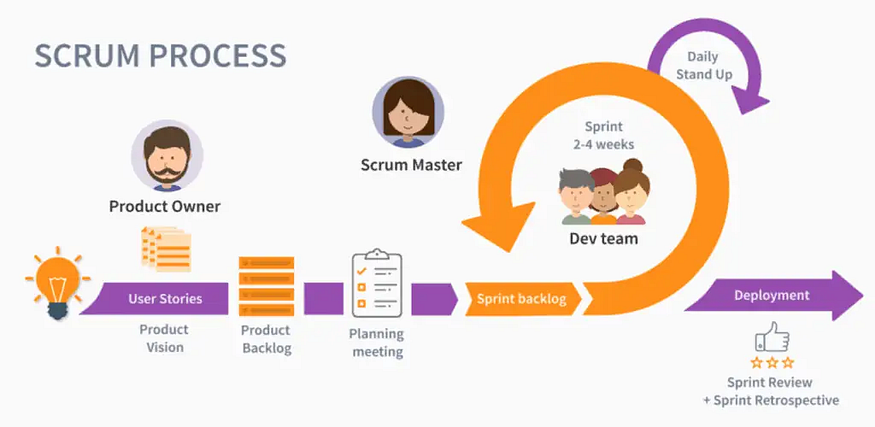
\includegraphics[width=0.8\columnwidth]{Processusde scrum.png}}
        \caption{Processus de Scrum}
        \label{fig:logo_tt}
    \end{figure}

\subsection{Langage de modélisation}

Le Unified Modeling Language (UML) a été conçu pour être un langage de modélisation visuel. Il est prévu pour l'architecture, la conception et l'implémentation de systèmes logiciels complexes par leur structure ainsi que leur  comportement. UML dispose d'applications qui vont au-delà du développement logiciel, en particulier pour les flux de processus dans l'industrie. Il ressemble aux plans utilisés dans d'autres domaines et se compose de différents types de diagrammes. D'une façon générale, les diagrammes UML décrivent les frontières, la structure et le comportement du système et de ses objets. \cite[]{UML}

\section*{Conclusion}

Dans cette section, nous avons introduit « Vermeg », notre organisme d’accueil. Ensuite, nous avons examiné les concepts clés liés aux API, réalisé une étude de marché, une étude de l’existant et enfin, argumenté du choix de la méthodologie de développement et du langage de modélisation .Dans le deuxième chapitre, nous aborderons la planification du projet. 


